To study the system behaviour in practice, we used real-world block data to simulate the operations and returns of a subscription contract. The source code of the simulation script is available in \href{https://github.com/giordano-lucas/refees/blob/simulation/Use_case_simulation.ipynb}{this GitHub repository}.
We assume that blocks are added approximately every 20 seconds to the Ethereum blockchain. Thus, there are roughly $b=\frac{24*3600}{20}=4320$ blocks created every day, and a month represent $129'000$ blocks.


Using this information, we initialise a contract with the values highlighted in table \ref{tab:variables:application-1}.

\begin{table}[htbp]
\caption{Smart contract variables}
\begin{center}
\begin{tabular}{|l|c|l|c|}
\hline
\textbf{Name} & Ref.& Value  \\
\hline
Maturity & $M$ & $60\cdot b \;(\sim 60 \,days)$\\
Payment frequency & $f$ & $10 \cdot b  \;(\sim 10 \,days)$  \\
Payment amount & $x$ & 4200000 Gwei \\
Initial reserve& $r$ & 30000000 Gwei \\
Max operations & $n_{ops}$ & \{"transfer": 20\} \\
Mean factor & $\alpha$ & 1 \\
\hline
\end{tabular}
\label{tab:variables:application-1}
\end{center}
\end{table}

For simplicity reasons, it is assumed that the client uses all the operations possible ($20$ transfers every $f$ blocks). We also assume that he uses the exact average gas price ($\alpha = 1$) for each of his operations. Moreover, the amount of gas used by a simple transfer can slightly vary because of how the Ethereum Virtual Machine (EVM) works but, in our simulation, we use a constant value for this number, namely: $n_{gas} = 21000$.


The parameters being set, we sample ($20$ every $f$ block) from real Ethereum data (from block 4000000 to block $4000000+M$) available at \cite{EthereumBlockData}. Figure \ref{fig:gas-price-no-outlier} contains a plot of the sampled data.
\begin{figure}[h]
\centering
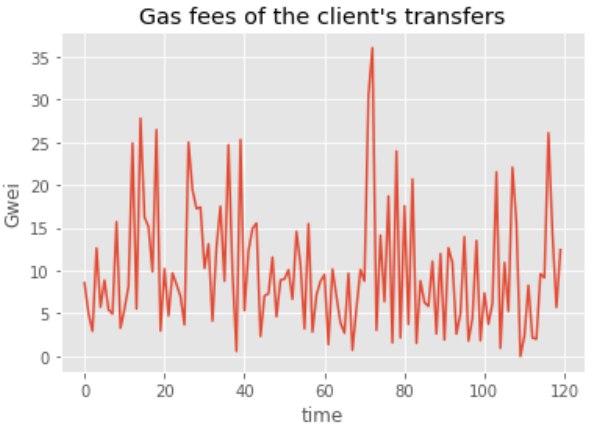
\includegraphics[scale=0.55]{figures/gas fees client transfer.png}
\label{fig:gas-price-no-outlier}
\end{figure}
Then, using this series of gas prices, we simulate the behaviour of the contract and report the returns in table \ref{tab:variables:application-2}. We observe that the provider makes a profit using the system. 

\begin{table}[htbp]
\caption{{\projectName} returns  (without outlier). }
\begin{center}
\begin{tabular}{|l|c|}
\hline
Gas used by the client & 0.02509 ETH \\
\hline
Total payments of the client & 0.0252 ETH \\
\hline
Client return &  0.02509-0.0252 = -0.00011 ETH \\
\hline
provider return &  0.0252-0.02509  = 0.00011 ETH \\
\hline
\end{tabular}
\label{tab:variables:application-2}
\end{center}
\end{table}
Furthermore, we repeat this simulation on the same data after including an outlier (gas price multiple times higher than average). This outlier also comes from the real-world data. It simulates the fact that the client operates when the network is busy. We obtain the gas prices shown in figure \ref{fig:gas-price-with-outlier}. Similarly, realised returns for both client and providers are reported in table \ref{tab:variables:application-3}. 

\begin{figure}[h]
\centering
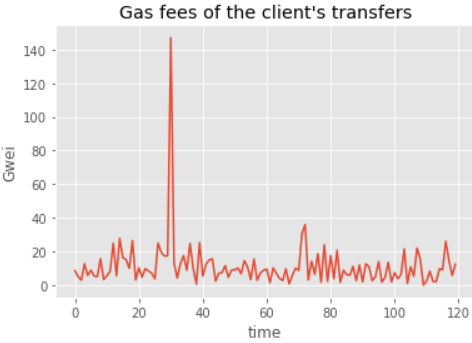
\includegraphics[scale=0.55]{figures/gas fees client transfer outlier.png}
\label{fig:gas-price-with-outlier}
\end{figure}


\begin{table}[htbp]
\caption{{\projectName} returns (with an outlier).}
\begin{center}
\begin{tabular}{|l|c|}
\hline
Gas used by the client & 0.02797 ETH \\
\hline
Total payments of the client & 0.0252 ETH \\
\hline
Client return &  0.02797-0.0252 = 0.00277 ETH \\
\hline
Provider return &  0.02509-0.0252  = -0.00277 ETH \\
\hline
\end{tabular}
\label{tab:variables:application-3}
\end{center}
\end{table}

When analysing these numbers, it appears that the system is only beneficial for one of the two actors, there is a winner and a loser. However, this example was the simplest possible. It will be shown in section \ref{section:future:gas-token} that it is possible to combine the system with \$GAS tokens to make it profitable for both actors.   